
%(BEGIN_QUESTION)
% Copyright 2007, Tony R. Kuphaldt, released under the Creative Commons Attribution License (v 1.0)
% This means you may do almost anything with this work of mine, so long as you give me proper credit

Endebrytere er elektriske brytere som er laget slik at de aktueres ved bevegelse eller posisjon til et objekt, istedenfor at et menneske skal trykke inn en knapp. Enkle endebrytere bruker direkte fysisk kontakt med en arm, og av og til en rulle på enden for lav friksjon. 

$$\includegraphics[width=15.5cm]{i02242x01.eps}$$

\vskip 30pt

Vis hvordan du ville koblet kretsen ovenfor slik av endebryeren slukker lyset når den aktueres. Lyset skal altså normalt være på. 

\underbar{file i02242}
%(END_QUESTION)





%(BEGIN_ANSWER)

$$\includegraphics[width=15.5cm]{i02242x02.eps}$$

%(END_ANSWER)





%(BEGIN_NOTES)


%INDEX% Switch, limit: mechanical actuation (direct contact)

%(END_NOTES)


